%!TEX root = documentation.tex

\chapter{Slave}

The term slave subsumes all parts of the sensor capturing unit.
The following explanations will discuss hardware and software individually to provide a more specific view of these parts.

\section{Hardware}

\begin{figure}[ht]
    \centering
    \subfloat[Sensor device with all cables connected]{\label{fig:sensordevice} 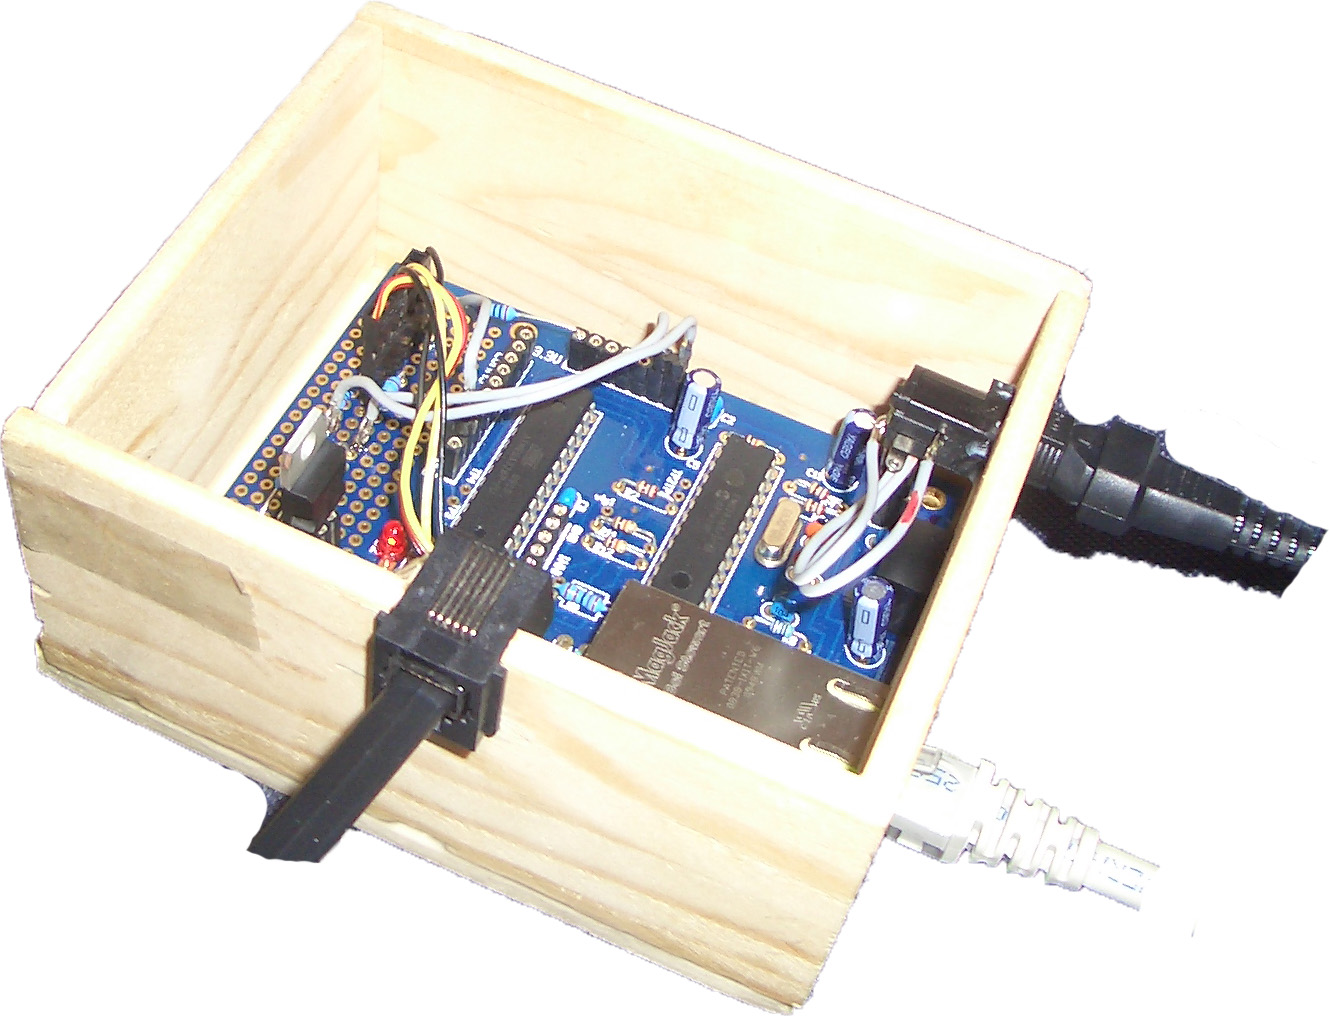
\includegraphics[width=0.5\linewidth]{graphics/sensordevice.jpg}}
    \qquad
    \subfloat[Mainboard with position of parts]{\label{fig:mainboard} 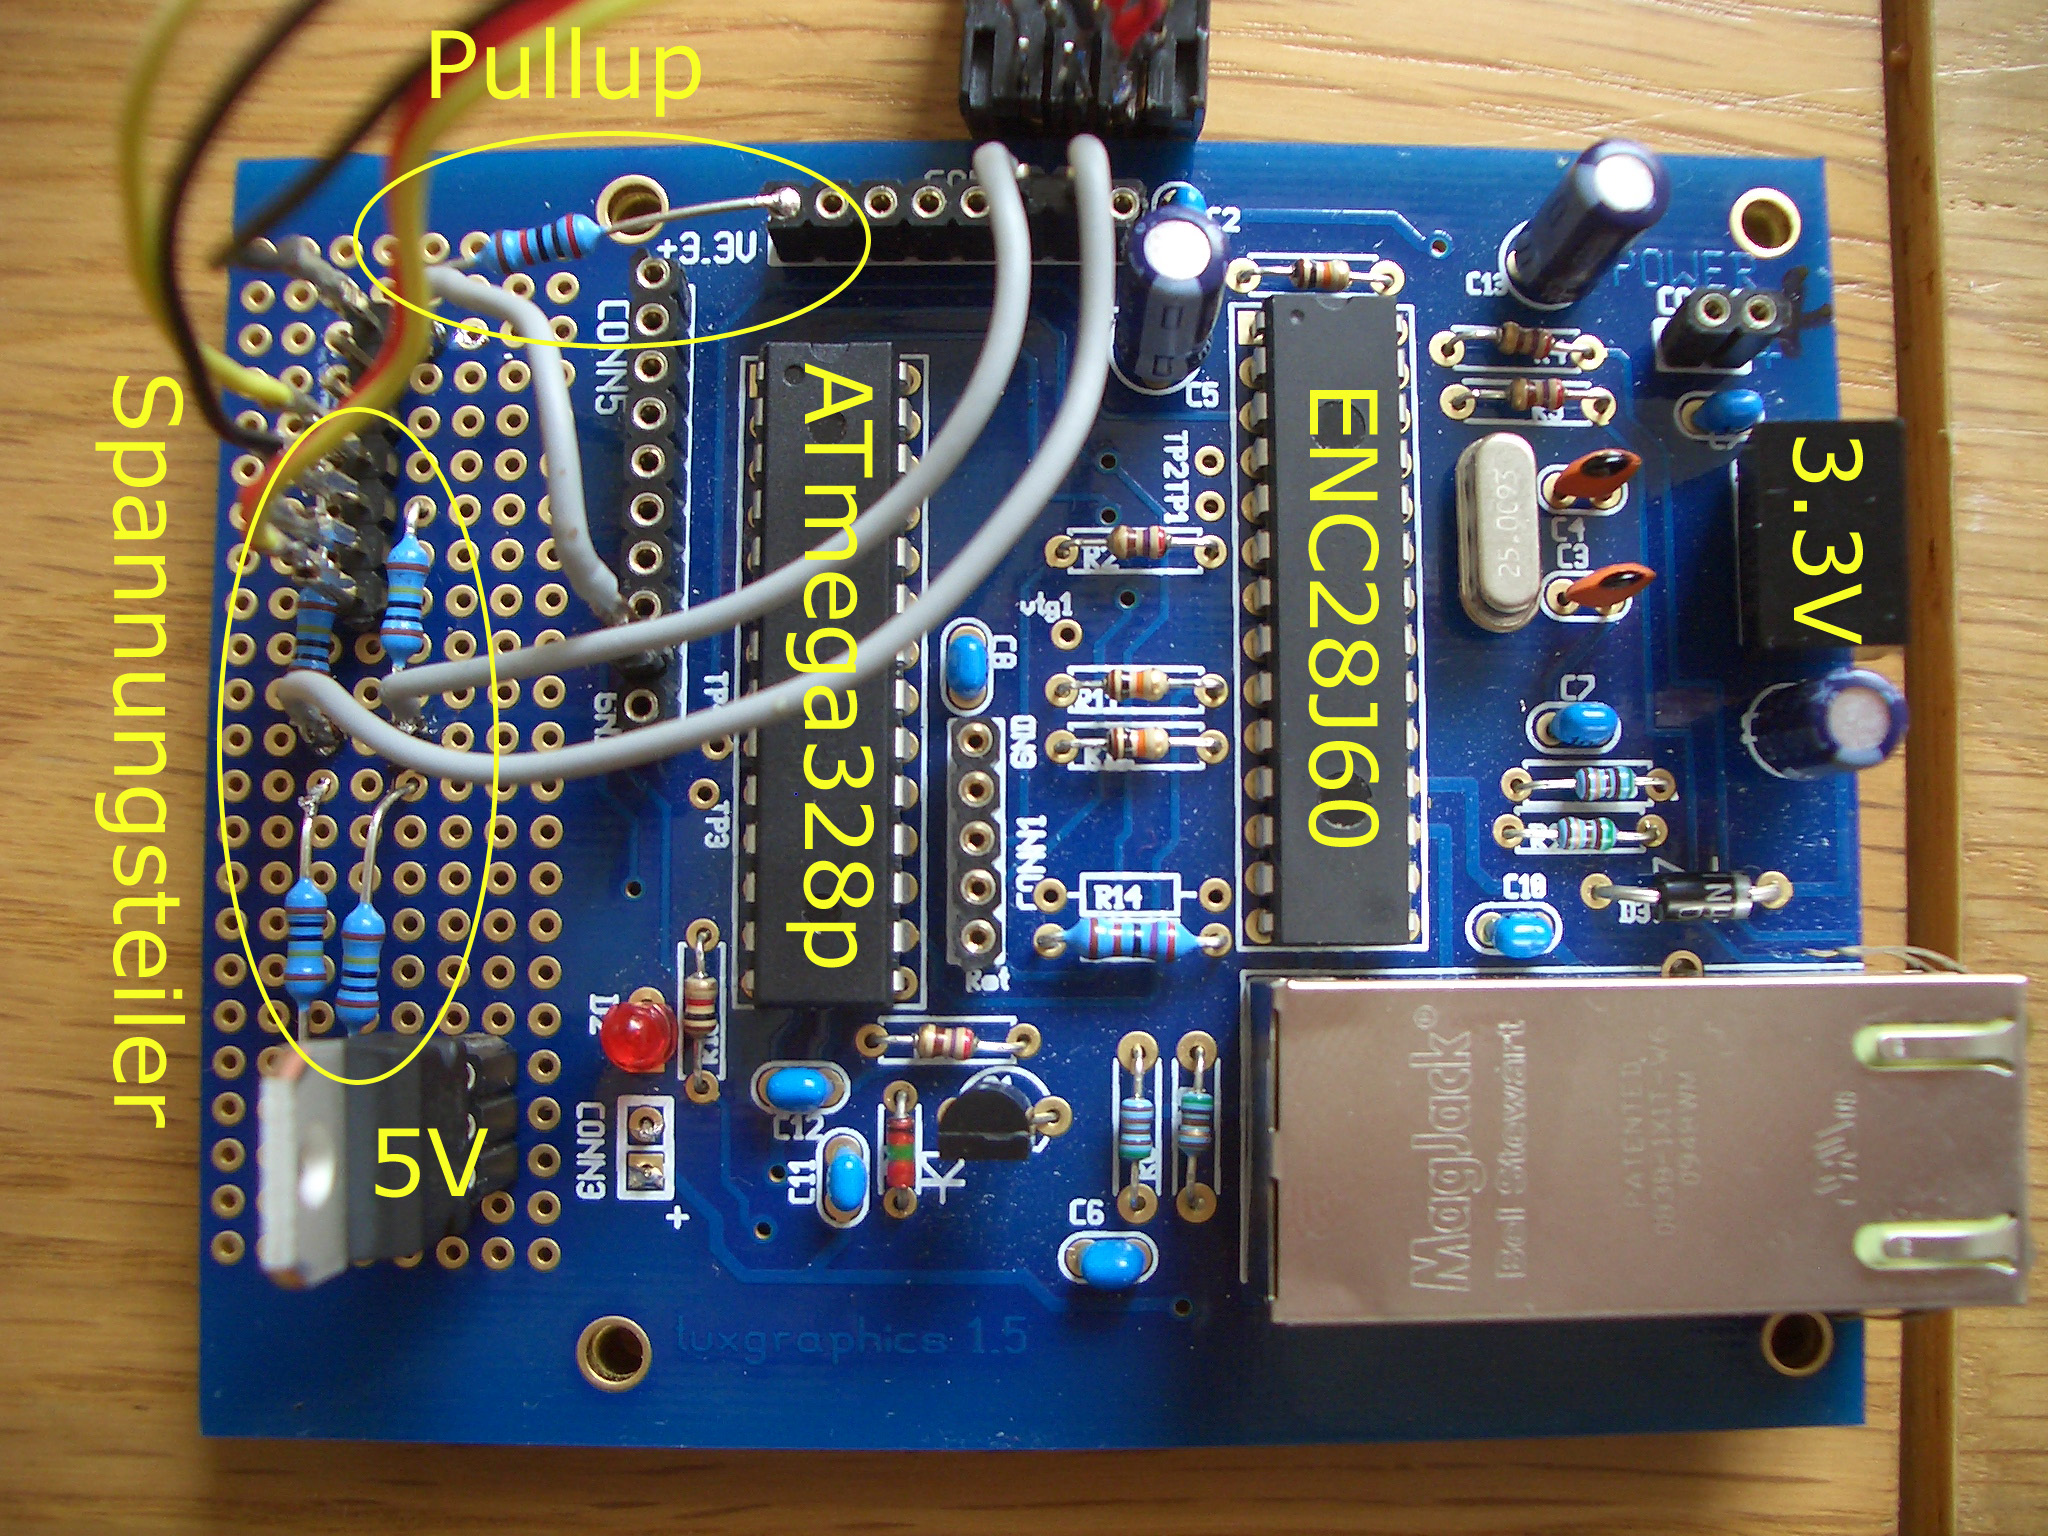
\includegraphics[width=0.5\linewidth]{graphics/mainboard.jpg}}
    \qquad
    \label{view:slave1}
\end{figure}

\begin{figure}[ht]
    \centering
    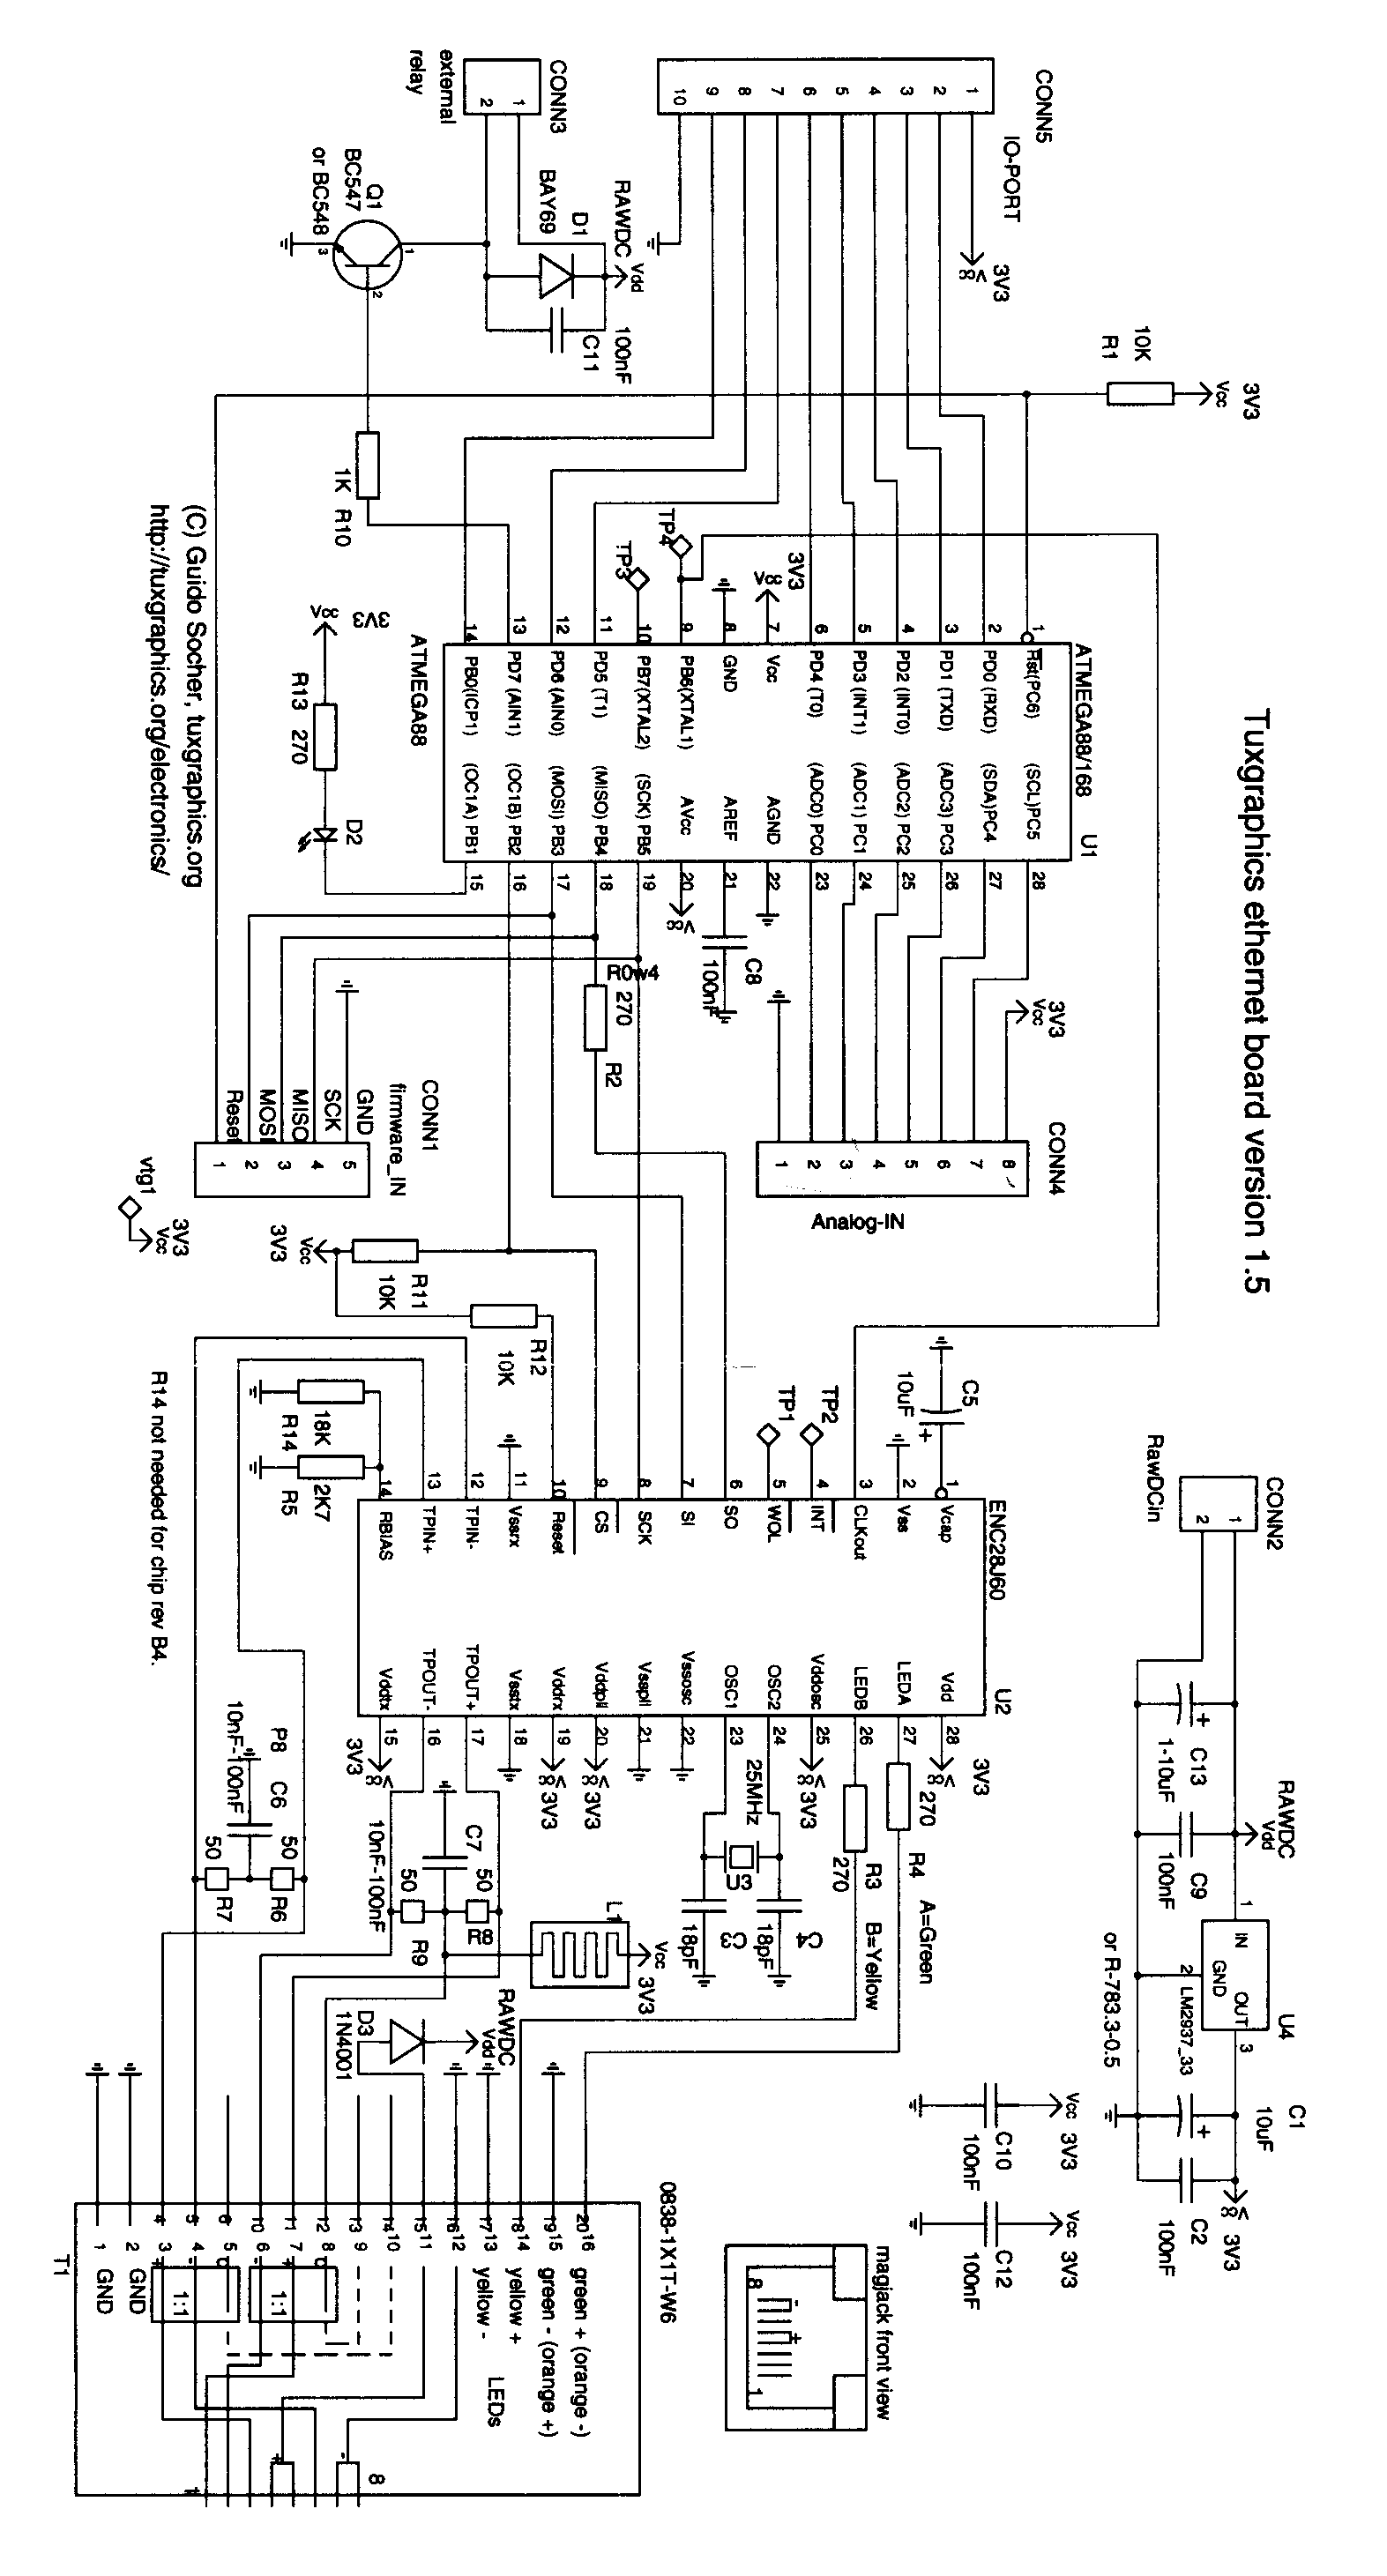
\includegraphics[width=0.7\linewidth]{graphics/schematics1.png}
    \caption{Schematics of mainboard}
    \label{fig:mainboard_schematic1}
\end{figure}

\begin{figure}[ht]
    \centering
    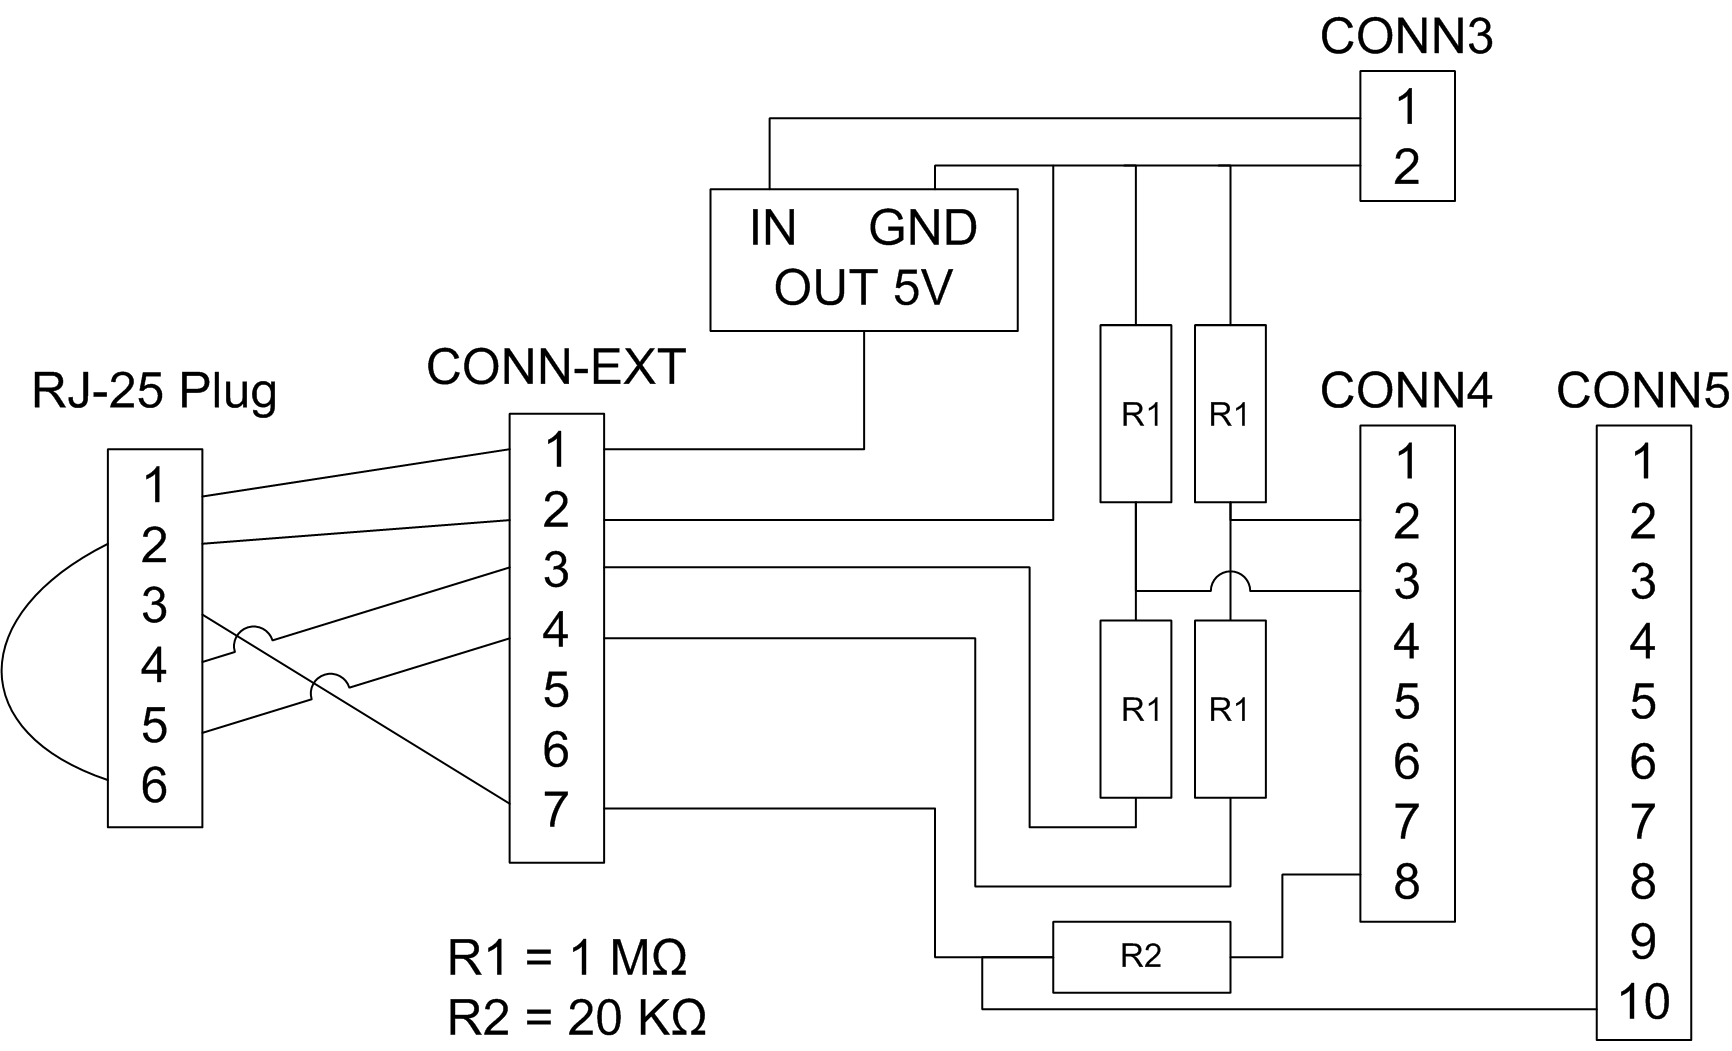
\includegraphics[width=\linewidth]{graphics/schematics.png}
    \caption{Schematics of additional hardware for sensor communication}
    \label{fig:mainboard_schematic}
\end{figure}

The measurement data acquisition and TCP/IP handling is done by an ATMEL ATmega328p chip, whereas the basic Ethernet communication is handled by an ENC28J60 chip from Microchip. Both chips are communicating via an SPI connection.\footnote{The mainboard is a product of \url{http://tuxgraphics.org}} 

The mainboard is operated at $3.3 V$ via a voltage regulator. Due to the fact that the sensor device requires a supply voltage of $5 V$, a separate voltage regulator has been added. This regulator is sourced by CONN3 of the mainboard which can be switch on and off by software via the transistor connected upstream.

To be able to process the analog signals from the sensor device at the ATmega328p, two 1:1 voltage dividers have been installed. This limits the maximum input voltage at the microcontroller's side to $2.5 V$.

The signal generated by the Reed contacts for capturing the wind speed is processed by using the Input Capture Unit of the microcontroller. The necessary pullup resistor is provided externally to ensure a fixed voltage reference. The internal pullup resistor may be too big due to production variations and may lead to undetectable signals.

The whole system runs at $12.5 MHz$ system clock speed.

\section{Software}

\begin{figure}[ht]
    \centering
    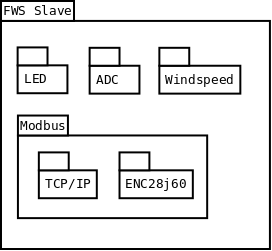
\includegraphics[width=0.6\linewidth]{graphics/fws_slave.png}
    \caption{Overview of software modules}
    \label{fig:slave_software}
\end{figure}

\subsection{Main FWS Slave module}
The main loop of the program uses polling to check for new data arriving from the Ethernet chip.

All other functionalities are implemented in submodules which are using interrupts and callback routines to return the results. In general, problems of parallel processes are avoided as interrupt routines cannot be interrupted.

\subsection{Modbus module}
In respect to the TCP/Modbus jargon the slave acts as a Server.

This module consists of two submodules which encapsulate the access to the ENC28J60 via SPI as well as the implementation of the protocols TCP/IP, ICMP and ARP. These submodules where taken from ,,tuxgraphics TCP/IP stack, 3rd generation'' \footnote{\url{http://tuxgraphics.org/common/src2/article09051/}}\footnote{\url{http://tuxgraphics.org/electronics/200905/embedded-tcp-ip-stack.shtml}} and adapted as needed.

The Modbus module itself is an in-house development. It currently supports the Modbus function codes for writing and reading single registers. It also has the possibility to request the device identifier. This function has not been implemented completely as the Java-Modbus-Library at the master does not provide this feature.

Registers (variables located in the main module) that should be available for Modbus transfers are registered using the module's API.

\subsection{Analog signals - Temperature and wind direction}
The Analog-Digital-Converter unit is encapsulated by the ADC sub module designed for subsequent capturing of multiple analog channels.
Since the ATmega328p has only one ADC unit just one channel can be converted at once.

As this application needs to sample two channels this has to be done one after the other. To ensure safe channel switching, the ADC unit is driven using single conversions with highest possible prescaler providing maximum resolution.

Naturally analog signals are subject to interference leading to non-precise results. In order to achieve a better data quality, the ADC module samples the current channel 256 times and calculates an average value before triggering the callback function and before switching to the next channel.

\subsection{Index signal - Wind speed}
The wind speed is triggered by a Reed contact in the sensor device generating a frequency of $2.53 Hz$ per $1 m/s$ wind speed.

This signal is captured using the Input Capture Unit of 16-bit Timer 1. Counting the elapsed time between two index pulses allows to calculate the actual wind speed. This wind speed module also includes specific limits for valid data. For instance, in cases where there's hardly any wind and the wind wheel comes to stop right on top of the Reed contact, input capture interrupts are triggered permanently causing the calculation result to reach unfeasible values. These cases can be avoided by dropping all results not matching the specified values of the wind speed sensor.

\section{Modbus Write Commands}
All described parameters are permanently saved to internal EEPROM. In case of EEPROM error they are reset to their default values. To modify the parameters, they can be transferred via Modbus commands (see address reference table \ref{tab:modbus_write}). All changes are stored in EEPROM automatically.

\begin{table}[ht]
    \centering
    \begin{tabular}{|l|l|l|l|}
    \hline \textbf{Address} & \textbf{Description} & \textbf{Valid values} & \textbf{Data format} \\ 
    \hline
    \hline 0 & IP address high segments & 16-bit unsigned & 65535 \\ 
    \hline 1 & IP address low segments & 16-bit unsigned & 65535 \\ 
    \hline 2 & Sensor enable & 0 (disable), 1 (enable) & 65535 \\ 
    \hline 3 & k high word & 16-bit unsigned & 65535 \\ 
    \hline 4 & k low word & 16-bit unsigned & 65535 \\ 
    \hline 5 & d high word & 16-bit unsigned & 65535 \\ 
    \hline 6 & d low word & 16-bit unsigned & 65535 \\ 
    \hline 7 & div high word & 16-bit unsigned & 65535 \\ 
    \hline 8 & div low word & 16-bit unsigned & 65535 \\ 
    \hline 
    \end{tabular}
    \caption{Modbus Write Addresses}
    \label{tab:modbus_write}
\end{table}

\subsection{Network}
The mainboard supports $10 Mbit/s$ T-Base Ethernet LAN. The user can change the IP address according to his needs. The port 502 is fixed and is reserved for Modbus communication by standards.

\begin{itemize}
    \item Possible values: any IP address (IPv4)
    \item Default value: 192.168.0.111
\end{itemize}

\paragraph{Write address: 0} 
\begin{itemize}
    \item Value high byte: First segment of IP address (e.g. 192)
    \item Value low byte: Second segment (e.g. 168)
\end{itemize}

\paragraph{Write address: 1} 
\begin{itemize}
    \item Value high byte: Third segment of IP address (e.g. 0)
    \item  Value low byte: Fourth segment (e.g. 111)
\end{itemize}

IP address change sequence: First write to address 0 then address to 1. Changes will take effect when the complete address has been received and Modbus response has been sent with the old IP address.

\subsection{Sensor enable}
\label{sec:sensor_enable}
The microcontroller has a configuration parameter for enabling/disabling the the sensor device completely by switching the connected transistor. 

\paragraph{Read and Write address: 2}
\paragraph{Possible values:}
\begin{itemize}
    \item 0 = disable
    \item 1 = enable (default)
\end{itemize}

\subsection{Temperature calibration}
The temperature calculation uses the following formula:
\[
Temperature = (k * Value_{sensor} + d) / div
\]
Where the factors k, d and div are responsible for calibration. Sensor values are between 0 and 720. All factors are 32-bit signed values. This means 2 transmission per factor are necessary starting at address 3 with high word of k.

\paragraph{Possible values:} any 32 bit signed value

\paragraph{Default values:}
\begin{itemize}
\item $k = -1134  $
\item $d = 690000 $
\item $div = 1000 $
\end{itemize}

\paragraph{Change sequence:} Always write all 3 factors with the high word in the order k, d and finally div. Changes will take effect when the lower word of div has been received.

\section{Modbus Read Commands}
The registers listed in table \ref{tab:modbus_read} show the available sensor data.

\begin{table}[ht]

    \centering
    \begin{tabular}{|l|l|l|l|}
    \hline \textbf{Address} & \textbf{Description} & \textbf{Valid values} & \textbf{Data format} \\ 
    \hline
    \hline 2 & Sensor enable & 0 (disable), 1 (enable) & 65535 \\ 
    \hline 3 & Wind direction & 0..3375 (steps of 225); 32767 = no value & 6553.5 \\ 
    \hline 4 & Wind speed & 0..1000 (steps of 1); 65535 = no value & 6553.5 \\ 
    \hline 5 & Temperature & 16-bit signed; 32767 = no value & 6553.5 \\ 
    \hline 
    \end{tabular}
    \caption{Modbus Read Addresses}
    \label{tab:modbus_read}
\end{table}

\subsection{Sensor enable}
Please refer to Section~\ref{sec:sensor_enable}.

\paragraph{Read address:} 2

\subsection{Wind direction}
This register holds the current wind direction in a range from $0 to 337.5$ degrees. As the sensor detects 16 positions the delivered value also has a step size of $22.5$ degrees.

The transferred value is multiplied by 10 to transmit the first decimal place.

The value 32767 is transferred if the slave has been disabled (refer to Section~\ref{sec:sensor_enable}).

\paragraph{Read address:} 3

\subsection{Wind speed}
The current wind speed is denoted by values within the range from 0 to 100.0.

The transferred value is multiplied by 10 to transmit the first decimal place.

The value 65535 is transferred if the slave has been disabled (refer to Section~\ref{sec:sensor_enable}).

\paragraph{Read address:} 4

\subsection{Temperature}
This register holds the current temperature. The range is only limited by the sensor (refer to Figure~\ref{fig:windsensor_spec}).

The transferred value is multiplied by 10 to transmit the first decimal place.

\paragraph{Read address:} 5

\newpage